\documentclass[]{tufte-handout}

% ams
\usepackage{amssymb,amsmath}

\usepackage{ifxetex,ifluatex}
\usepackage{fixltx2e} % provides \textsubscript
\ifnum 0\ifxetex 1\fi\ifluatex 1\fi=0 % if pdftex
  \usepackage[T1]{fontenc}
  \usepackage[utf8]{inputenc}
\else % if luatex or xelatex
  \makeatletter
  \@ifpackageloaded{fontspec}{}{\usepackage{fontspec}}
  \makeatother
  \defaultfontfeatures{Ligatures=TeX,Scale=MatchLowercase}
  \makeatletter
  \@ifpackageloaded{soul}{
     \renewcommand\allcapsspacing[1]{{\addfontfeature{LetterSpace=15}#1}}
     \renewcommand\smallcapsspacing[1]{{\addfontfeature{LetterSpace=10}#1}}
   }{}
  \makeatother

\fi

% graphix
\usepackage{graphicx}
\setkeys{Gin}{width=\linewidth,totalheight=\textheight,keepaspectratio}

% booktabs
\usepackage{booktabs}

% url
\usepackage{url}

% hyperref
\usepackage{hyperref}

% units.
\usepackage{units}


\setcounter{secnumdepth}{-1}

% citations

\newlength{\cslhangindent}
\setlength{\cslhangindent}{1.5em}
% For Pandoc 2.8 to 2.11
\newenvironment{cslreferences}%
  {}%
  {\par}
% For pandoc 2.11+ using new --citeproc
\newlength{\csllabelwidth}
\setlength{\csllabelwidth}{3em}
\newenvironment{CSLReferences}[3] % #1 hanging-ident, #2 entry spacing
 {% don't indent paragraphs
  \setlength{\parindent}{0pt}
  % turn on hanging indent if param 1 is 1
  \ifodd #1 \everypar{\setlength{\hangindent}{\cslhangindent}}\ignorespaces\fi
  % set entry spacing
  \ifnum #2 > 0
  \setlength{\parskip}{#2\baselineskip}
  \fi
 }%
 {}
\usepackage{calc}
\newcommand{\CSLBlock}[1]{#1\hfill\break}
\newcommand{\CSLLeftMargin}[1]{\parbox[t]{\csllabelwidth}{#1}}
\newcommand{\CSLRightInline}[1]{\parbox[t]{\linewidth - \csllabelwidth}{#1}}
\newcommand{\CSLIndent}[1]{\hspace{\cslhangindent}#1}

% pandoc syntax highlighting
\usepackage{color}
\usepackage{fancyvrb}
\newcommand{\VerbBar}{|}
\newcommand{\VERB}{\Verb[commandchars=\\\{\}]}
\DefineVerbatimEnvironment{Highlighting}{Verbatim}{commandchars=\\\{\}}
% Add ',fontsize=\small' for more characters per line
\newenvironment{Shaded}{}{}
\newcommand{\AlertTok}[1]{\textcolor[rgb]{1.00,0.00,0.00}{\textbf{#1}}}
\newcommand{\AnnotationTok}[1]{\textcolor[rgb]{0.38,0.63,0.69}{\textbf{\textit{#1}}}}
\newcommand{\AttributeTok}[1]{\textcolor[rgb]{0.49,0.56,0.16}{#1}}
\newcommand{\BaseNTok}[1]{\textcolor[rgb]{0.25,0.63,0.44}{#1}}
\newcommand{\BuiltInTok}[1]{#1}
\newcommand{\CharTok}[1]{\textcolor[rgb]{0.25,0.44,0.63}{#1}}
\newcommand{\CommentTok}[1]{\textcolor[rgb]{0.38,0.63,0.69}{\textit{#1}}}
\newcommand{\CommentVarTok}[1]{\textcolor[rgb]{0.38,0.63,0.69}{\textbf{\textit{#1}}}}
\newcommand{\ConstantTok}[1]{\textcolor[rgb]{0.53,0.00,0.00}{#1}}
\newcommand{\ControlFlowTok}[1]{\textcolor[rgb]{0.00,0.44,0.13}{\textbf{#1}}}
\newcommand{\DataTypeTok}[1]{\textcolor[rgb]{0.56,0.13,0.00}{#1}}
\newcommand{\DecValTok}[1]{\textcolor[rgb]{0.25,0.63,0.44}{#1}}
\newcommand{\DocumentationTok}[1]{\textcolor[rgb]{0.73,0.13,0.13}{\textit{#1}}}
\newcommand{\ErrorTok}[1]{\textcolor[rgb]{1.00,0.00,0.00}{\textbf{#1}}}
\newcommand{\ExtensionTok}[1]{#1}
\newcommand{\FloatTok}[1]{\textcolor[rgb]{0.25,0.63,0.44}{#1}}
\newcommand{\FunctionTok}[1]{\textcolor[rgb]{0.02,0.16,0.49}{#1}}
\newcommand{\ImportTok}[1]{#1}
\newcommand{\InformationTok}[1]{\textcolor[rgb]{0.38,0.63,0.69}{\textbf{\textit{#1}}}}
\newcommand{\KeywordTok}[1]{\textcolor[rgb]{0.00,0.44,0.13}{\textbf{#1}}}
\newcommand{\NormalTok}[1]{#1}
\newcommand{\OperatorTok}[1]{\textcolor[rgb]{0.40,0.40,0.40}{#1}}
\newcommand{\OtherTok}[1]{\textcolor[rgb]{0.00,0.44,0.13}{#1}}
\newcommand{\PreprocessorTok}[1]{\textcolor[rgb]{0.74,0.48,0.00}{#1}}
\newcommand{\RegionMarkerTok}[1]{#1}
\newcommand{\SpecialCharTok}[1]{\textcolor[rgb]{0.25,0.44,0.63}{#1}}
\newcommand{\SpecialStringTok}[1]{\textcolor[rgb]{0.73,0.40,0.53}{#1}}
\newcommand{\StringTok}[1]{\textcolor[rgb]{0.25,0.44,0.63}{#1}}
\newcommand{\VariableTok}[1]{\textcolor[rgb]{0.10,0.09,0.49}{#1}}
\newcommand{\VerbatimStringTok}[1]{\textcolor[rgb]{0.25,0.44,0.63}{#1}}
\newcommand{\WarningTok}[1]{\textcolor[rgb]{0.38,0.63,0.69}{\textbf{\textit{#1}}}}

% longtable

% multiplecol
\usepackage{multicol}

% strikeout
\usepackage[normalem]{ulem}

% morefloats
\usepackage{morefloats}


% tightlist macro required by pandoc >= 1.14
\providecommand{\tightlist}{%
  \setlength{\itemsep}{0pt}\setlength{\parskip}{0pt}}

% title / author / date
\title{Einführung}
\author{true}
\date{2021-03-03}


\begin{document}

\maketitle




\hypertarget{klassische-frequentistische-statistik}{%
\section{Klassische (frequentistische)
Statistik}\label{klassische-frequentistische-statistik}}

Im Verlauf Ihres bisherigen Studiums haben Sie verschiedene statistische
Methode kennengelernt, die alle etwas mit \textbf{N}ull
\textbf{H}ypothesis \textbf{S}ignificance \textbf{T}esting (NHST) zu
haben. Diese Verfahren haben gemeinsam, dass sie

\begin{itemize}
\tightlist
\item
  Punktschätzungen von Parametern benutzen
\item
  mit diesen Punktschätzungen eine Teststatistik erstellen
\item
  die Wahrscheinlichkeit angeben, mit derer eine mindestens so extreme
  Ausprägung dieser Teststatistik erreicht wird, unter der Annahme, dass
  die Nullhypothese wahr ist. Diese Wahrscheinlichkeit nennt man einen
  \emph{p-Wert}.
\end{itemize}

Diese Methoden stehen schon seit längerem in der Kritik:

\begin{itemize}
\item
  Gigerenzer (2004);Gigerenzer (2018) behauptet unter anderem, dass die
  Verwendung von NHST Methoden oftmals einem statistischen Ritual
  gleichkommt.
\item
  Wasserstein and Lazar (2016) schreiben im \emph{Statement on
  Statistical Significance and P-Values} der American Statistical
  Association:

  \begin{itemize}
  \tightlist
  \item
    P-values can indicate how incompatible the data are with a specified
    statistical model.
  \item
    P-values do not measure the probability that the studied hypothesis
    is true, or the probability that the data were produced by random
    chance alone.
  \item
    Scientific conclusions and business or policy decisions should not
    be based only on whether a p-value passes a specific threshold.
  \end{itemize}
\end{itemize}

Es scheint also grosse Probleme mit dem Verständnis von Konzepten der
klassischen Statistik zu geben. Zum Beispiel werden Grundlegende
Konzepte wie p-Werte und Konfidenzintervalle oft falsch verstanden
(Hoekstra et al. 2014).

\hypertarget{beispiel-t-test}{%
\subsection{Beispiel: t-Test}\label{beispiel-t-test}}

Schauen wir uns das Beispiel der letzten Sitzung nochmals an. Wir haben
einen Datensatz generiert, um zwei geschätzte Mittelwerte zu
vergleichen, mit dem Ziel herauszufinden, ob eine Gruppe einen grösseren
Mittelwert als die andere hat.

\begin{Shaded}
\begin{Highlighting}[]
\FunctionTok{library}\NormalTok{(tidyverse)}
\FunctionTok{library}\NormalTok{(kableExtra)}
\end{Highlighting}
\end{Shaded}

\begin{verbatim}
## 
## Attaching package: 'kableExtra'
\end{verbatim}

\begin{verbatim}
## The following object is masked from 'package:dplyr':
## 
##     group_rows
\end{verbatim}

\begin{Shaded}
\begin{Highlighting}[]
\FunctionTok{set.seed}\NormalTok{(}\DecValTok{12}\NormalTok{)}

\CommentTok{\# Number of people wearing fancy hats}
\NormalTok{N\_fancyhats }\OtherTok{\textless{}{-}} \DecValTok{50} 

\CommentTok{\# Number of people not wearing fancy hats}
\NormalTok{N\_nofancyhats }\OtherTok{\textless{}{-}} \DecValTok{50}

\CommentTok{\# Population mean of creativity for people wearing fancy hats}
\NormalTok{mu\_fancyhats }\OtherTok{\textless{}{-}} \DecValTok{103} 

\CommentTok{\# Population mean of creativity for people wearing no fancy hats}
\NormalTok{mu\_nofancyhats }\OtherTok{\textless{}{-}} \DecValTok{98} 

\CommentTok{\# Average population standard deviation of both groups}
\NormalTok{sigma }\OtherTok{\textless{}{-}} \DecValTok{15} 

\CommentTok{\# Generate data}
\NormalTok{fancyhats }\OtherTok{=} \FunctionTok{tibble}\NormalTok{(}\AttributeTok{Creativity =} \FunctionTok{rnorm}\NormalTok{(N\_fancyhats, mu\_fancyhats, sigma),}
               \AttributeTok{Group =} \StringTok{"Fancy Hat"}\NormalTok{)}

\NormalTok{nofancyhats }\OtherTok{=} \FunctionTok{tibble}\NormalTok{(}\AttributeTok{Creativity =} \FunctionTok{rnorm}\NormalTok{(N\_nofancyhats, mu\_nofancyhats, sigma),}
                 \AttributeTok{Group =} \StringTok{"No Fancy Hat"}\NormalTok{)}


\NormalTok{FancyHat }\OtherTok{\textless{}{-}} \FunctionTok{bind\_rows}\NormalTok{(fancyhats, nofancyhats)  }\SpecialCharTok{\%\textgreater{}\%}
    \FunctionTok{mutate}\NormalTok{(}\AttributeTok{Group =} \FunctionTok{fct\_relevel}\NormalTok{(}\FunctionTok{as.factor}\NormalTok{(Group), }\StringTok{"No Fancy Hat"}\NormalTok{))}
\end{Highlighting}
\end{Shaded}

Die Daten sehen so aus:

\begin{Shaded}
\begin{Highlighting}[]
\FunctionTok{kbl}\NormalTok{(FancyHat) }\SpecialCharTok{\%\textgreater{}\%}
  \FunctionTok{kable\_paper}\NormalTok{() }\SpecialCharTok{\%\textgreater{}\%}
  \FunctionTok{scroll\_box}\NormalTok{(}\AttributeTok{width =} \StringTok{"500px"}\NormalTok{, }\AttributeTok{height =} \StringTok{"200px"}\NormalTok{)}
\end{Highlighting}
\end{Shaded}

\begin{table}
\centering
\begin{tabular}[t]{r|l}
\hline
Creativity & Group\\
\hline
80.79149 & Fancy Hat\\
\hline
126.65754 & Fancy Hat\\
\hline
88.64883 & Fancy Hat\\
\hline
89.19992 & Fancy Hat\\
\hline
73.03537 & Fancy Hat\\
\hline
98.91556 & Fancy Hat\\
\hline
98.26977 & Fancy Hat\\
\hline
93.57617 & Fancy Hat\\
\hline
101.40304 & Fancy Hat\\
\hline
109.42022 & Fancy Hat\\
\hline
91.33421 & Fancy Hat\\
\hline
83.59177 & Fancy Hat\\
\hline
91.30650 & Fancy Hat\\
\hline
103.17928 & Fancy Hat\\
\hline
100.71376 & Fancy Hat\\
\hline
92.44804 & Fancy Hat\\
\hline
120.83319 & Fancy Hat\\
\hline
108.10768 & Fancy Hat\\
\hline
110.60452 & Fancy Hat\\
\hline
98.60042 & Fancy Hat\\
\hline
106.35462 & Fancy Hat\\
\hline
133.10802 & Fancy Hat\\
\hline
118.17969 & Fancy Hat\\
\hline
98.46311 & Fancy Hat\\
\hline
87.62133 & Fancy Hat\\
\hline
98.98923 & Fancy Hat\\
\hline
100.01342 & Fancy Hat\\
\hline
104.96684 & Fancy Hat\\
\hline
105.18700 & Fancy Hat\\
\hline
108.43097 & Fancy Hat\\
\hline
113.10972 & Fancy Hat\\
\hline
134.08054 & Fancy Hat\\
\hline
94.88457 & Fancy Hat\\
\hline
86.94262 & Fancy Hat\\
\hline
97.41315 & Fancy Hat\\
\hline
95.72288 & Fancy Hat\\
\hline
107.12176 & Fancy Hat\\
\hline
95.80731 & Fancy Hat\\
\hline
114.97158 & Fancy Hat\\
\hline
87.93323 & Fancy Hat\\
\hline
104.57476 & Fancy Hat\\
\hline
85.66011 & Fancy Hat\\
\hline
111.67202 & Fancy Hat\\
\hline
79.06562 & Fancy Hat\\
\hline
98.37245 & Fancy Hat\\
\hline
109.74199 & Fancy Hat\\
\hline
88.34420 & Fancy Hat\\
\hline
105.84997 & Fancy Hat\\
\hline
113.97180 & Fancy Hat\\
\hline
95.61101 & Fancy Hat\\
\hline
97.35973 & No Fancy Hat\\
\hline
96.30994 & No Fancy Hat\\
\hline
104.85241 & No Fancy Hat\\
\hline
128.30502 & No Fancy Hat\\
\hline
82.23665 & No Fancy Hat\\
\hline
109.01978 & No Fancy Hat\\
\hline
106.08875 & No Fancy Hat\\
\hline
78.28591 & No Fancy Hat\\
\hline
94.24942 & No Fancy Hat\\
\hline
102.71307 & No Fancy Hat\\
\hline
104.09820 & No Fancy Hat\\
\hline
112.91631 & No Fancy Hat\\
\hline
110.83653 & No Fancy Hat\\
\hline
100.95693 & No Fancy Hat\\
\hline
110.51488 & No Fancy Hat\\
\hline
110.70185 & No Fancy Hat\\
\hline
127.31158 & No Fancy Hat\\
\hline
65.76110 & No Fancy Hat\\
\hline
112.56680 & No Fancy Hat\\
\hline
115.17592 & No Fancy Hat\\
\hline
90.11899 & No Fancy Hat\\
\hline
101.75480 & No Fancy Hat\\
\hline
91.55890 & No Fancy Hat\\
\hline
95.26221 & No Fancy Hat\\
\hline
96.45034 & No Fancy Hat\\
\hline
88.49243 & No Fancy Hat\\
\hline
78.93419 & No Fancy Hat\\
\hline
92.24074 & No Fancy Hat\\
\hline
105.75134 & No Fancy Hat\\
\hline
95.33047 & No Fancy Hat\\
\hline
98.06387 & No Fancy Hat\\
\hline
78.88911 & No Fancy Hat\\
\hline
94.96834 & No Fancy Hat\\
\hline
115.46699 & No Fancy Hat\\
\hline
97.64931 & No Fancy Hat\\
\hline
111.45735 & No Fancy Hat\\
\hline
95.34913 & No Fancy Hat\\
\hline
114.70564 & No Fancy Hat\\
\hline
89.87167 & No Fancy Hat\\
\hline
83.54903 & No Fancy Hat\\
\hline
103.64673 & No Fancy Hat\\
\hline
83.22989 & No Fancy Hat\\
\hline
111.46339 & No Fancy Hat\\
\hline
99.93894 & No Fancy Hat\\
\hline
113.50554 & No Fancy Hat\\
\hline
92.86566 & No Fancy Hat\\
\hline
104.78422 & No Fancy Hat\\
\hline
87.57893 & No Fancy Hat\\
\hline
94.41480 & No Fancy Hat\\
\hline
82.89052 & No Fancy Hat\\
\hline
\end{tabular}
\end{table}

Und grafisch dargestellt (als Boxplot):

\begin{Shaded}
\begin{Highlighting}[]
\CommentTok{\# plot both groups}
\NormalTok{FancyHat }\SpecialCharTok{\%\textgreater{}\%} 
    \FunctionTok{ggplot}\NormalTok{() }\SpecialCharTok{+}
    \FunctionTok{geom\_boxplot}\NormalTok{ ((}\FunctionTok{aes}\NormalTok{(}\AttributeTok{y =}\NormalTok{ Creativity, }\AttributeTok{x =}\NormalTok{ Group))) }\SpecialCharTok{+}
    \FunctionTok{labs}\NormalTok{(}\AttributeTok{title=} \StringTok{"Box Plot of Creativity Values"}\NormalTok{) }\SpecialCharTok{+}
    \FunctionTok{theme\_bw}\NormalTok{()}
\end{Highlighting}
\end{Shaded}

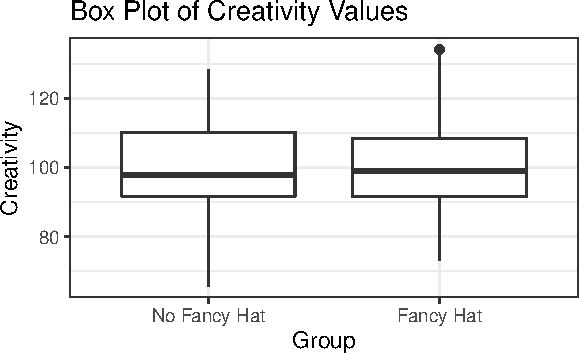
\includegraphics{01-intro-bayesian-stats_files/figure-latex/unnamed-chunk-3-1}

Unter der Annahme, dass die beiden Gruppen dieselbe Standardabweichung
haben, machen wir einen t-Test:

\begin{Shaded}
\begin{Highlighting}[]
\NormalTok{fancyhat\_ttest }\OtherTok{\textless{}{-}} \FunctionTok{t.test}\NormalTok{(Creativity }\SpecialCharTok{\textasciitilde{}}\NormalTok{ Group,}
       \AttributeTok{var.equal =} \ConstantTok{TRUE}\NormalTok{,}
       \AttributeTok{data =}\NormalTok{ FancyHat)}
\end{Highlighting}
\end{Shaded}

\begin{Shaded}
\begin{Highlighting}[]
\NormalTok{fancyhat\_ttest\_tab }\OtherTok{\textless{}{-}}\NormalTok{ broom}\SpecialCharTok{::}\FunctionTok{tidy}\NormalTok{(fancyhat\_ttest)}
\end{Highlighting}
\end{Shaded}

\begin{Shaded}
\begin{Highlighting}[]
\NormalTok{fancyhat\_ttest\_tab }\SpecialCharTok{\%\textgreater{}\%}
    \FunctionTok{select}\NormalTok{(estimate, estimate1, estimate2, statistic, p.value, conf.low, conf.high) }\SpecialCharTok{\%\textgreater{}\%}
    \FunctionTok{round}\NormalTok{(}\DecValTok{3}\NormalTok{) }\SpecialCharTok{\%\textgreater{}\%} 
    \FunctionTok{kbl}\NormalTok{() }\SpecialCharTok{\%\textgreater{}\%}
    \FunctionTok{kable\_classic}\NormalTok{(}\AttributeTok{full\_width =} \ConstantTok{FALSE}\NormalTok{, }\AttributeTok{html\_font =} \StringTok{"Cambria"}\NormalTok{)}
\end{Highlighting}
\end{Shaded}

\begin{table}
\centering
\begin{tabular}[t]{r|r|r|r|r|r|r}
\hline
estimate & estimate1 & estimate2 & statistic & p.value & conf.low & conf.high\\
\hline
-1.647 & 99.209 & 100.856 & -0.637 & 0.526 & -6.78 & 3.486\\
\hline
\end{tabular}
\end{table}

Es ist vielleicht nicht ganz offensichtlich, dass wir hier mehrere Dinge
gemacht haben:

\begin{enumerate}
\def\labelenumi{\arabic{enumi})}
\item
  Wir haben zwei Mittelwerte geschätzt. Genauer gesagt haben wir zwei
  Punktschätzungen der Gruppenmittelwerte\footnote{\texttt{estimate1}
    und \texttt{estimate2}}.
\item
  Wir schätzen die resultierende Differenz der
  Gruppenmittelwerte\footnote{\texttt{estimate}}.
\item
  Wir berechnen eine Teststatistik (empirischer t-Wert)\footnote{\texttt{statistic}}.
\item
  Wir berechnen die Wahrscheinlichkeit, unter der Nullhypothese einen
  t-Wert zu erhalten, der einen mindestens so grossen Betrag hat wie der
  empirische t-Wert\footnote{\texttt{p.value}}.
\end{enumerate}

Diskutieren Sie die Bedeutung des erhalten p-Wertes und des
Konfidenzintervalles. Finden Sie diese Konzepte intuitiv verständlich?
Können Sie erklären, was ein Konfidenzintervall ist?

Der p-Wert beträgt 0.53. Was können wir damit anfangen?

\hypertarget{weitere-probleme}{%
\subsection{Weitere Probleme}\label{weitere-probleme}}

Es gibt viele weitere Probleme mit dem frequentistischen Ansatz
(Wagenmakers 2007)---die oben genannten haben damit zu tun, dass die
Konzepte nicht sonderlich intuitiv sind. Wir hätten z.B. gerne die
Wahrscheinlichkeit, mit der eine Hypothese wahr/falsch ist.

frequentische Statistik kann eine solche Aussage prinzipiell nicht
machen.

Ein weiteres Problem ist, dass Anreize in der Forschung oftmals dazu
verleiten, frequentistische NHST falsch einzusetzen. Verschiedene
\emph{bad practices} sind unter dem Begriff \textbf{p-hacking} bekannt.
Damit kann z.B. gemeint sein, viele Hypothesentests durchzuführen, aber
nur diejenigen zu Berichten, welche ein signifikantes Resultat ergeben.

Schlussendlich ist auch so, dass frequentistische Statistik nicht den
von den Axiomen der Wahrscheinlichkeitstheorie Gebrauch macht, um
Parameter zu schätzen, und die Unsicherheit bei der Schätzung nicht
anhand einer Wahrscheinlichkeitsverteilung quantifiziert.

\hypertarget{philosophie-der-wahrscheinlichkeit}{%
\subsection{Philosophie der
Wahrscheinlichkeit}\label{philosophie-der-wahrscheinlichkeit}}

In der klassischen Statistik wird Wahrscheinlichkeit als relative
Häufigkeits eines Ereignisses verstanden. Dies bedeutet, dass nur
Ereignisse, welche (unendlich) oft wiederholt werden können, eine
Wahrscheinlichkeit haben können.

Somit ist es unmöglich, dass Parameter oder Hypothesen eine
Wahrscheinlichkeitsverteilung haben können. Zum Vergleich von
frequentistischer und Bayesianischer Auffassung von Wahrscheinlichkeiten
gibt es
\href{https://de.wikipedia.org/wiki/Frequentistischer_Wahrscheinlichkeitsbegriff}{hier}
und
\href{https://de.wikipedia.org/wiki/Bayessche_Statistik\#Der_bayessche_Wahrscheinlichkeitsbegriff}{hier}
mehr Information.

\hypertarget{bayesianische-statistik}{%
\section{Bayesianische Statistik}\label{bayesianische-statistik}}

\hypertarget{degrees-of-belief}{%
\subsection{Degrees of belief}\label{degrees-of-belief}}

Wir werden nun mit einem anderen Ansatz arbeiten. Dieser beruht auf den
Axiomen der Wahrscheinlichkeitstheorie, und auf der Auffassung von
Wahrscheinlichkeit als \textbf{degree of belief}, also vom der Grad
persönlichen Überzeugung. Daher wird dieser Ansatz of \emph{subjektiv}
genannt.

Meiner Meinung nach ist diese philosophische Diskussion über
Interpretationen der Wahrscheinlichkeitstheorie nicht besonders
zielführend. Wir können die unterschiedlichen Meinungen einfach zur
Kenntnis nehmen.

Die wichtigste Erkenntnis ist jedenfalls:
Wahrscheinlichkeitsverteilungen quantifizieren unseren Wissensstand,
oder genauer gesagt, unsere Unsicherheit (uncertainty) über etwas. Dies
kann eine Aussage sein, wie z.B. ``es wird morgen regnen,'' oder ein
Parameter in einem statistischen Modell, oder eine Hypothese.

Die in @ref(fig:gamma-dist) abgebildeten Verteilungen zeigen unsere
Unsicherheit über eine Variable \(x\). Wir wissen, dass \(x>0\), und wir
vermuten, dass \(x<50\). In einem Fall (violette Verteilung) glauben wir
sogar mit einiger Sicherheit, dass \(x<10\).

\begin{Shaded}
\begin{Highlighting}[]
\FunctionTok{library}\NormalTok{(tidyverse)}

\FunctionTok{tibble}\NormalTok{(}\AttributeTok{x =} \FunctionTok{seq}\NormalTok{(}\AttributeTok{from =} \DecValTok{0}\NormalTok{, }\AttributeTok{to =} \DecValTok{60}\NormalTok{, }\AttributeTok{by =}\NormalTok{ .}\DecValTok{1}\NormalTok{)) }\SpecialCharTok{\%\textgreater{}\%} 
  \FunctionTok{expand}\NormalTok{(x, }\FunctionTok{nesting}\NormalTok{(}\AttributeTok{alpha =} \FunctionTok{c}\NormalTok{(}\DecValTok{2}\NormalTok{, }\DecValTok{4}\NormalTok{), }
                    \AttributeTok{beta  =} \FunctionTok{c}\NormalTok{(}\FloatTok{0.1}\NormalTok{, }\DecValTok{1}\NormalTok{))) }\SpecialCharTok{\%\textgreater{}\%} 
  \FunctionTok{mutate}\NormalTok{(}\AttributeTok{density =} \FunctionTok{dgamma}\NormalTok{(x, alpha, beta),}
         \AttributeTok{group   =} \FunctionTok{rep}\NormalTok{(letters[}\DecValTok{1}\SpecialCharTok{:}\DecValTok{2}\NormalTok{], }\AttributeTok{times =} \FunctionTok{n}\NormalTok{() }\SpecialCharTok{/} \DecValTok{2}\NormalTok{)) }\SpecialCharTok{\%\textgreater{}\%} 
  
  \FunctionTok{ggplot}\NormalTok{(}\FunctionTok{aes}\NormalTok{(}\AttributeTok{x =}\NormalTok{ x, }\AttributeTok{ymin =} \DecValTok{0}\NormalTok{, }\AttributeTok{ymax =}\NormalTok{ density, }
             \AttributeTok{group =}\NormalTok{ group, }\AttributeTok{fill =}\NormalTok{ group)) }\SpecialCharTok{+}
  \FunctionTok{geom\_ribbon}\NormalTok{(}\AttributeTok{size =} \DecValTok{0}\NormalTok{, }\AttributeTok{alpha =} \DecValTok{3}\SpecialCharTok{/}\DecValTok{4}\NormalTok{) }\SpecialCharTok{+}
  \FunctionTok{scale\_fill\_viridis\_d}\NormalTok{(}\AttributeTok{option =} \StringTok{"B"}\NormalTok{, }\AttributeTok{direction =} \SpecialCharTok{{-}}\DecValTok{1}\NormalTok{, }
                       \AttributeTok{begin =} \DecValTok{1}\SpecialCharTok{/}\DecValTok{3}\NormalTok{, }\AttributeTok{end =} \DecValTok{2}\SpecialCharTok{/}\DecValTok{3}\NormalTok{) }\SpecialCharTok{+}
  \FunctionTok{scale\_x\_continuous}\NormalTok{(}\AttributeTok{expand =} \FunctionTok{expansion}\NormalTok{(}\AttributeTok{mult =} \FunctionTok{c}\NormalTok{(}\DecValTok{0}\NormalTok{, }\FloatTok{0.05}\NormalTok{))) }\SpecialCharTok{+}
  \FunctionTok{scale\_y\_continuous}\NormalTok{(}\ConstantTok{NULL}\NormalTok{, }\AttributeTok{breaks =} \ConstantTok{NULL}\NormalTok{) }\SpecialCharTok{+}
  \FunctionTok{coord\_cartesian}\NormalTok{(}\AttributeTok{xlim =} \FunctionTok{c}\NormalTok{(}\DecValTok{0}\NormalTok{, }\DecValTok{50}\NormalTok{)) }\SpecialCharTok{+}
  \FunctionTok{theme}\NormalTok{(}\AttributeTok{panel.grid =} \FunctionTok{element\_blank}\NormalTok{(),}
        \AttributeTok{legend.position =} \StringTok{"none"}\NormalTok{)}
\end{Highlighting}
\end{Shaded}

\begin{figure}
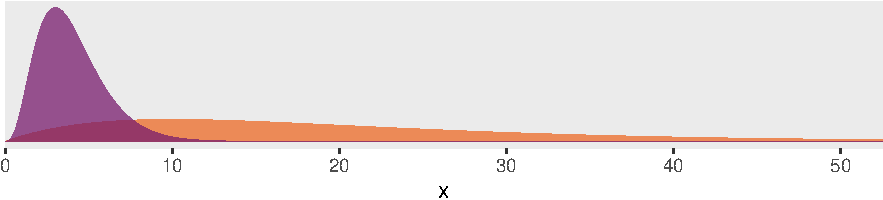
\includegraphics{01-intro-bayesian-stats_files/figure-latex/gamma-dist-1} \caption[Wahrscheinlichkeitsverteilungen]{Wahrscheinlichkeitsverteilungen}\label{fig:gamma-dist}
\end{figure}

In der Bayesianischen Statistik erhalten wir anstatt Punktschätzungen
von Parametern ganze Verteilungen, mit denen wir unsere Unsicherheit
quantifizieren. Ganz stark vereinfacht brauchen wir in der
Bayesianischen Statistik eine Prior-Verteilung Englisch: \emph{prior}),
und wir erhalten eine Posteriori-Verteilung (Englisch:
\emph{posterior}), nachdem wir unseren prior anhand der Daten
(\emph{likelihood}) angepasst haben.

Unser \textbf{prior} gibt an, was wir glauben, bevor wir die Daten
berücksichtigen, und unser \textbf{posterior} gibt an, was wir glauben,
nachdem wir die Daten gesehen haben.

Bayesianische Statistik erfordert also ein paar neue Konzepte, aber
längerfristig ist dieser Ansatz einfacher, denn es beruht alles auf ein
paar wenigen Grundsätzen.

Die Vorteile des Bayesianischen Ansatzes sind:

\begin{itemize}
\item
  intuitiveres Verständnis von Unsicherheit.
\item
  erlaubt es uns Evidenz für oder gegen Hypothesen zu quantifizieren.
\item
  dieser Ansatz ist viel flexibler.
\item
  Wir können unser Wissen in Form von a priori-Verteilungen
  miteinbeziehen.
\item
  besser geeignet für Multilevel Modelle.
\end{itemize}

Bayesianische Statistik hat aber auch Nachteile:

\begin{itemize}
\item
  wir brauchen leistungsstarke Computer.
\item
  setzt Familiarität mit Wahrscheinlichkeitsverteilungen voraus.
\item
  es ist nicht einfach, Hypothesentests durchzuführen. Siehe z.B.
  \href{https://statmodeling.stat.columbia.edu/2017/05/04/hypothesis-testing-hint-not-think/}{hier}
  und
  \href{https://statmodeling.stat.columbia.edu/2011/04/02/so-called_bayes/}{hier}.
\end{itemize}

Warum brauchen wir viel Rechenpower, um Bayesianische Statistik zu
machen?

Dies hat damit zu tun, dass es nur in ganz wenigen Fällen einfach ist,
posterior Verteilungen zu erhalten. In wenigen Fällen ist es möglich,
diese analytisch zu bestimmen, in den den meisten Fällen brauchen wir
simulationsbasierte Sampling-Verfahren (Markov Chain Monte Carlo
Sampling), um die komplexen Wahrscheinlichkeitsverteilungen zu schätzen.
Dies erfordert sehr schnelle Prozessoren, und war deshalb in der
Vergangenheit nur auf Supercomputern möglich.

Das ist einer der wichtigsten Gründe, weshalb die frequentistische
Statistik so lange die einzige anwendbare Lösung war.

Wir werden nun anhand zweier einfacher Beispiele die Bayesianische
Parameterschätzung kennenlernen. Danach werden wir komplexere Beispiele
betrachten, und Methoden kennenlernen, mit denen wir Hypothesen testen
können. Hypothesentests sind eine Form von Modellvergleichen, und hier
gibt es mehrere Möglichkeit.

Wir werden machen, was Gigerenzer (2018) verlangt, und einen
\textbf{statistical toolkit} lernen, der weit über den Einsatz von
\emph{Ritualen} hinausgeht!

\hypertarget{grundlagen-der-bayesianischen-inferenz}{%
\subsection{Grundlagen der Bayesianischen
Inferenz}\label{grundlagen-der-bayesianischen-inferenz}}

\hypertarget{parameter-sind-zufallsvariablen}{%
\subsubsection{Parameter sind
Zufallsvariablen}\label{parameter-sind-zufallsvariablen}}

\begin{itemize}
\item
  Parameters sind Zufallsvariablen, im Gegensatz zum frequentistischen
  Ansatz, in dem Parameter keine Verteilung haben können.
\item
  Parameter kommen aus Wahrscheinlichkeitsverteilung, welche unser
  Wissen (Unsicherheit) repräsentieren
\item
  Die Prior-Verteilung wird anhand der Likelihood (Daten)
  \emph{updated}, um ein Posterior-Verteilung zu erhalten.
\end{itemize}

\hypertarget{drei-schritte-der-bayesianischen-datenanalyse}{%
\subsubsection{Drei Schritte der Bayesianischen
Datenanalyse}\label{drei-schritte-der-bayesianischen-datenanalyse}}

Im Prinzip folgt Bayesianische Datenanalyse immer den folgenden drei
Schritten:

\begin{enumerate}
\def\labelenumi{\arabic{enumi}.}
\item
  Wir schreiben ein Wahrscheinlichkeitsmodell auf, bestehen aus einer
  gemeinsamen Verteilung der beobachtent Variablen (\(y\), \(x\)) und
  der latenten Parameter \(\theta\)).
\item
  Wir berechnen die Posterior-Verteilung
  \(P(θ | y) \sim P(y | \theta) \cdot p(\theta)\), bedingt auf die
  beobachteten Daten.
\item
  Wir evaluieren das Modell und die Posterior-Verteilung.

  \begin{itemize}
  \tightlist
  \item
    Wie gut passt das Modell?
  \item
    Sind unsere Schlussfolgerungen gerechtfertigt?
  \item
    Wie empfindlich sind unsere Schätzungen gegenüber unseren Annahmen?
  \item
    Müssen wir unser Modell revidieren?
  \item
    Wir können anhand von Modellvergleichen Hypothesen testen.
  \end{itemize}
\end{enumerate}

\hypertarget{parameterschuxe4tzung-wahrscheinlichkeitsparameter-einer-binomialverteilung}{%
\subsection{Parameterschätzung: Wahrscheinlichkeitsparameter einer
Binomialverteilung}\label{parameterschuxe4tzung-wahrscheinlichkeitsparameter-einer-binomialverteilung}}

Wir schauen uns nun diesen Prozess anhand eines simplen Beispiels an.

\hypertarget{beispiel}{%
\subsubsection{Beispiel}\label{beispiel}}

Zwei Kartenspieler spielen gegeneinander. Sie beobachten, dass Spielerin
A 6 von 9 Spielen gewinnt, während Spielerin B nur 3 davon gewinnt. Sie
fragen sich nun, ob das nur Glück ist, oder ob Spielerin A tatsächlich
besser sein könnte.

Dieses Beispiel ist analytisch lösbar. Ich werde die analytische Lösung
in einem Blog Post demonstrieren, da wir hier eine simulationsbasierte
Lösung anstreben.

Wenn Sie diesen Sachverhalt quantifizieren möchten, könnten Sie
behaupten, dass die Wahrscheinlichkeit, dass Spielerin A gewinnt,
grösser als 0.5 sein müsste, falls diese besser ist. Eine
Wahrscheinlichkeit von 0.5 würde bedeuten, dass beide mit gleicher
Wahrscheinlichkeit gewinnen.

Unser Ziel ist es also, den Wahrscheinlichkeitsparameter \(\theta\)
einer Binomialverteilung zu schätzen. Die Daten, \(y\), sind in diesem
Fall die 6 Erfolge in 9 Versuchen.

\begin{Shaded}
\begin{Highlighting}[]
\NormalTok{wins }\OtherTok{\textless{}{-}} \DecValTok{6}
\NormalTok{games }\OtherTok{\textless{}{-}} \DecValTok{9}
\end{Highlighting}
\end{Shaded}

Wir wissen, dass die Anzahl Erfolge in k Spielen einer
Binomialverteilung folgt. Falls beide Spielerinnen gleich gut sind,
sollte die Erfolgswahrscheinlichkeit ungefähr 0.5 sein. Wir können die
Wahrscheinlichkeit berechnen, dass Spielerin A durch Glück 6 Spiele
gewinnt, d.h. unter der Annahme, dass beide gleich gut sind.

\begin{Shaded}
\begin{Highlighting}[]
\FunctionTok{dbinom}\NormalTok{(}\AttributeTok{x =}\NormalTok{ wins, }\AttributeTok{size =}\NormalTok{ games, }\AttributeTok{prob =} \FloatTok{0.5}\NormalTok{)}
\end{Highlighting}
\end{Shaded}

\begin{verbatim}
## [1] 0.1640625
\end{verbatim}

Diese Wahrscheinlichkeit ist ziemlich hoch. Wir können auch die
kumulative Wahrscheinlichkeit berechnen, 5 mal oder weniger zu gewinnen:

\begin{Shaded}
\begin{Highlighting}[]
\FunctionTok{pbinom}\NormalTok{(}\AttributeTok{q =} \DecValTok{5}\NormalTok{, }\AttributeTok{size =}\NormalTok{ games, }\AttributeTok{prob =} \FloatTok{0.5}\NormalTok{)}
\end{Highlighting}
\end{Shaded}

\begin{verbatim}
## [1] 0.7460937
\end{verbatim}

Die Wahrscheinlichkeit, 6, 7, 8 oder 9 mal zu gewinnen wäre demnach:

\begin{Shaded}
\begin{Highlighting}[]
\DecValTok{1} \SpecialCharTok{{-}} \FunctionTok{pbinom}\NormalTok{(}\AttributeTok{q =} \DecValTok{5}\NormalTok{, }\AttributeTok{size =}\NormalTok{ games, }\AttributeTok{prob =} \FloatTok{0.5}\NormalTok{)}
\end{Highlighting}
\end{Shaded}

\begin{verbatim}
## [1] 0.2539063
\end{verbatim}

oder

\begin{Shaded}
\begin{Highlighting}[]
\FunctionTok{pbinom}\NormalTok{(}\AttributeTok{q =} \DecValTok{5}\NormalTok{, }\AttributeTok{size =}\NormalTok{ games, }\AttributeTok{prob =} \FloatTok{0.5}\NormalTok{, }\AttributeTok{lower.tail =} \ConstantTok{FALSE}\NormalTok{)}
\end{Highlighting}
\end{Shaded}

\begin{verbatim}
## [1] 0.2539063
\end{verbatim}

Was haben wir hier berechnet? Was könnten wir hier mit einem
frequentistischen Ansatz machen?

Wir können aber auch eine Punktschätzung der Wahrscheinlichkeit
erhalten.

\begin{Shaded}
\begin{Highlighting}[]
\NormalTok{theta }\OtherTok{\textless{}{-}}\NormalTok{ wins}\SpecialCharTok{/}\NormalTok{games}
\NormalTok{theta}
\end{Highlighting}
\end{Shaded}

\begin{verbatim}
## [1] 0.6666667
\end{verbatim}

Dies entspricht derjenigen Schätzung, für welche die Wahrscheinlichkeit
maximiert wird, diese Daten zu beobachten. Dies nennt man eine
\textbf{Maximum Likelihood} Schätzung.

\begin{Shaded}
\begin{Highlighting}[]
\FunctionTok{tibble}\NormalTok{(}\AttributeTok{x =} \FunctionTok{seq}\NormalTok{(}\AttributeTok{from =} \DecValTok{0}\NormalTok{, }\AttributeTok{to =} \DecValTok{1}\NormalTok{, }\AttributeTok{by =}\NormalTok{ .}\DecValTok{01}\NormalTok{)) }\SpecialCharTok{\%\textgreater{}\%} 
  \FunctionTok{mutate}\NormalTok{(}\AttributeTok{density =} \FunctionTok{dbinom}\NormalTok{(}\DecValTok{6}\NormalTok{, }\DecValTok{9}\NormalTok{, x)) }\SpecialCharTok{\%\textgreater{}\%} 
  
  \FunctionTok{ggplot}\NormalTok{(}\FunctionTok{aes}\NormalTok{(}\AttributeTok{x =}\NormalTok{ x, }\AttributeTok{ymin =} \DecValTok{0}\NormalTok{, }\AttributeTok{ymax =}\NormalTok{ density)) }\SpecialCharTok{+}
  \FunctionTok{geom\_ribbon}\NormalTok{(}\AttributeTok{size =} \DecValTok{0}\NormalTok{, }\AttributeTok{alpha =} \DecValTok{1}\SpecialCharTok{/}\DecValTok{4}\NormalTok{, }\AttributeTok{fill =} \StringTok{"steelblue"}\NormalTok{) }\SpecialCharTok{+}
  \FunctionTok{geom\_vline}\NormalTok{(}\AttributeTok{xintercept =}\NormalTok{ theta, }\AttributeTok{linetype =} \DecValTok{2}\NormalTok{, }\AttributeTok{size =} \FloatTok{1.2}\NormalTok{) }\SpecialCharTok{+}
  \FunctionTok{scale\_y\_continuous}\NormalTok{(}\ConstantTok{NULL}\NormalTok{, }\AttributeTok{breaks =} \ConstantTok{NULL}\NormalTok{) }\SpecialCharTok{+}
  \FunctionTok{coord\_cartesian}\NormalTok{(}\AttributeTok{xlim =} \FunctionTok{c}\NormalTok{(}\DecValTok{0}\NormalTok{, }\DecValTok{1}\NormalTok{)) }\SpecialCharTok{+}
  \FunctionTok{xlab}\NormalTok{(}\StringTok{"Wahrscheinlichkeit"}\NormalTok{) }\SpecialCharTok{+}
  \FunctionTok{theme}\NormalTok{(}\AttributeTok{panel.grid =} \FunctionTok{element\_blank}\NormalTok{(),}
        \AttributeTok{legend.position =} \StringTok{"none"}\NormalTok{)}
\end{Highlighting}
\end{Shaded}

\begin{figure}
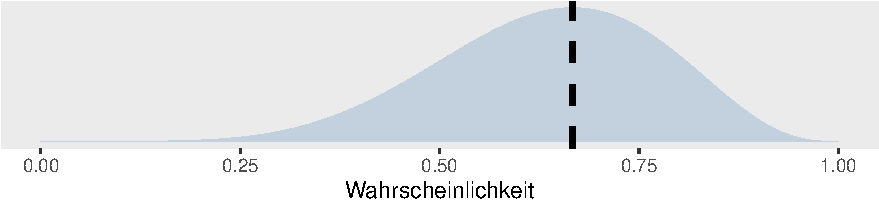
\includegraphics{01-intro-bayesian-stats_files/figure-latex/maxlikbinom-1} \caption[Maximum-Likelihood Schätzung ]{Maximum-Likelihood Schätzung }\label{fig:maxlikbinom}
\end{figure}

Grafik @ref(fig:maxlikbinom) zeigt, dass \(\theta\) = 6/9 derjenige
Parameter ist, für den die Wahrscheinlichkeit maximiert wird, dass wir 6
Erfolge in 9 Spielen beobachten.

\hypertarget{bayes-theorem}{%
\subsection{Bayes' Theorem}\label{bayes-theorem}}

Mit einer Punktschätzung können wir unsere Unsicherheit aber nicht
quantifizieren---dafür brauchen wir eine Verteilung über den ganzen
Bereich der möglichen Parameterwerte. Diese Verteilung erhalten wir,
indem wir das Bayes'sche Theorem anwenden. Die Wahrscheinlichkeit, dass
A gewinnt, \(\theta\), bedingt auf die Daten, ist:

\[ P(\theta|Data) = \frac{ P(Data|\theta) * P(\theta) } {P(Data)}\] Der
Term \(P(Data)\) ist eingentlich nur eine Normalisierungskonstante,
welche dafür sorgt, dass wir eine Verteilung erhalten (welche zu 1
integriert), und wird oft weggelassen:

\[ P(\theta|Data) \propto P(Data|\theta) * P(\theta) \] Um dies zu
berechnen, brauchen wir \(P(Data|\theta)\) und \(P(\theta)\).
\(P(Data|\theta)\) ist einfach; die Wahrscheinlichkeit \(k\) Erfolge in
\(n\) Versuchen zu erhalten ist

\[ P(x = k) = {n \choose k} \theta^k (1-\theta^{n-k}) \] Das bedeutet:
\(k\) Erfolge mit Wahrscheinlichkeit \(\theta^k\) und \(n-k\)
Misserfolge mit Wahrscheinlichkeit \(1-\theta^{n-k}\). Mit dem Term
\(\binom{n}{k} = \frac{n!}{k!(n-k)!}\) berücksichtigen wir alle
Reihenfolgen, mit denen wir 6 Erfolge in 9 Spielen erhalten.

\(P(\theta)\) ist die a-priori-Wahrscheinlichkeit, mit der Spielerin A
gewinnt. Wenn wir nicht über die beiden Spielerinnen wissen, ist es
sinnvoll anzunehmen, dass alle Wahrscheinlichkeiten zwischen 0 und 1
gleichwahrscheinlich sind. So eine Verteilung nennt man eine uniforme
Verteilung über dem Interval
\(\left(0, 1\right) = \{x \in \mathbb{R} | 0 < x < 1 \}\).

Wir definieren nun einen Vektor von möglichen Werten:

\begin{Shaded}
\begin{Highlighting}[]
\NormalTok{n\_points }\OtherTok{\textless{}{-}} \DecValTok{100}
\NormalTok{p\_grid }\OtherTok{\textless{}{-}} \FunctionTok{seq}\NormalTok{( }\AttributeTok{from=}\DecValTok{0}\NormalTok{ , }\AttributeTok{to=}\DecValTok{1}\NormalTok{ , }\AttributeTok{length.out =}\NormalTok{ n\_points )}
\end{Highlighting}
\end{Shaded}

Die Likelihood, das heisst die Wahrscheinlichkeit der Daten für jeden
möglichen Parameterwert, ist

\begin{Shaded}
\begin{Highlighting}[]
\NormalTok{likelihood }\OtherTok{\textless{}{-}} \FunctionTok{dbinom}\NormalTok{(wins , }\AttributeTok{size =}\NormalTok{ games , }\AttributeTok{prob =}\NormalTok{ p\_grid)}
\end{Highlighting}
\end{Shaded}

\begin{Shaded}
\begin{Highlighting}[]
\NormalTok{compute\_posterior }\OtherTok{=} \ControlFlowTok{function}\NormalTok{(likelihood, prior)\{}
  \CommentTok{\# compute product of likelihood and prior}
\NormalTok{  unstandardized\_posterior }\OtherTok{\textless{}{-}}\NormalTok{ likelihood }\SpecialCharTok{*}\NormalTok{ prior}
  
  \CommentTok{\# standardize the posterior, so it sums to 1}
\NormalTok{  posterior }\OtherTok{\textless{}{-}}\NormalTok{ unstandardized\_posterior }\SpecialCharTok{/} \FunctionTok{sum}\NormalTok{(unstandardized\_posterior)}
  
  \FunctionTok{par}\NormalTok{(}\AttributeTok{mfrow=}\FunctionTok{c}\NormalTok{(}\DecValTok{1}\NormalTok{, }\DecValTok{3}\NormalTok{))}
  \FunctionTok{plot}\NormalTok{(p\_grid , prior, }\AttributeTok{type=}\StringTok{"l"}\NormalTok{, }\AttributeTok{main=}\StringTok{"Prior"}\NormalTok{, }\AttributeTok{col =} \StringTok{"dodgerblue3"}\NormalTok{, }\AttributeTok{lwd =} \DecValTok{2}\NormalTok{)}
  \FunctionTok{plot}\NormalTok{(p\_grid , likelihood, }\AttributeTok{type=}\StringTok{"l"}\NormalTok{, }\AttributeTok{main=}\StringTok{"Likelihood"}\NormalTok{, }\AttributeTok{col =} \StringTok{"firebrick3"}\NormalTok{, }\AttributeTok{lwd =} \DecValTok{2}\NormalTok{)}
  \FunctionTok{plot}\NormalTok{(p\_grid , posterior , }\AttributeTok{type=}\StringTok{"l"}\NormalTok{, }\AttributeTok{main=}\StringTok{"Posterior"}\NormalTok{, }\AttributeTok{col =} \StringTok{"darkorchid3"}\NormalTok{, }\AttributeTok{lwd =} \DecValTok{2}\NormalTok{)}
\NormalTok{\}}
\end{Highlighting}
\end{Shaded}

\begin{Shaded}
\begin{Highlighting}[]
\NormalTok{prior1 }\OtherTok{\textless{}{-}} \FunctionTok{rep}\NormalTok{(}\FloatTok{0.5}\NormalTok{ , }\FunctionTok{length}\NormalTok{(p\_grid))}
\FunctionTok{compute\_posterior}\NormalTok{(likelihood, prior1)}
\end{Highlighting}
\end{Shaded}

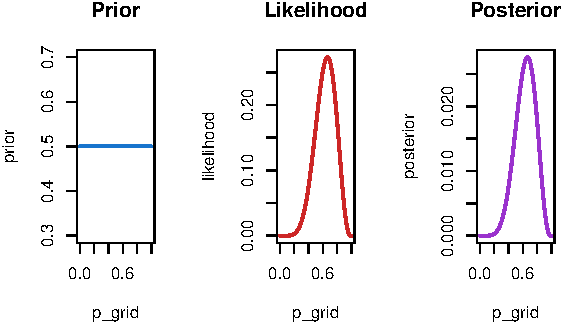
\includegraphics{01-intro-bayesian-stats_files/figure-latex/unnamed-chunk-17-1}

Da wir jeden Wert für gleich wahrscheinlich hielten, hat unser Prior
keinen Einfluss auf den Posterior.

Wir können aber unser Vorwissen auch anders ausdrücken. Vielleicht
halten wir es für möglich, dass A besser ist als B, aber wir glauben, es
sei unmöglich, dass B besser ist. Dieser Glaube könnte durch folgenden
Prior repräsentiert werden.

\begin{Shaded}
\begin{Highlighting}[]
\NormalTok{prior2 }\OtherTok{\textless{}{-}} \FunctionTok{ifelse}\NormalTok{(p\_grid }\SpecialCharTok{\textless{}} \FloatTok{0.5}\NormalTok{ , }\DecValTok{0}\NormalTok{ , }\DecValTok{1}\NormalTok{)}
\FunctionTok{compute\_posterior}\NormalTok{(likelihood, prior2)}
\end{Highlighting}
\end{Shaded}

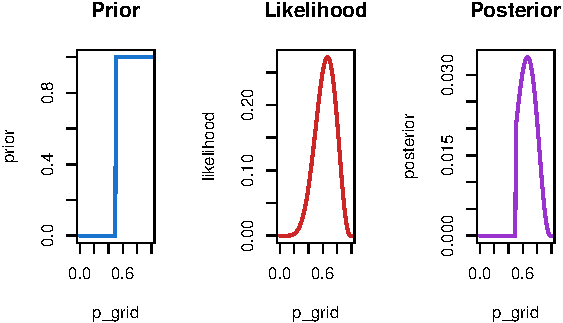
\includegraphics{01-intro-bayesian-stats_files/figure-latex/unnamed-chunk-18-1}
Dies führt dazu, dass in unserem Posterior Werte \(< 0.5\) nicht möglich
sind, weil wir dieses Vorwissen in unserem Prior spezifiziert hatten.

Wir können aber auch abenteuerliche Priors benutzen, wie z.B. folgender:
Wir glauben, dass \(0.5\) der wahrscheinlichste Wert ist, mit einem
exponentiellen Abfall auf beide Seiten.

\begin{Shaded}
\begin{Highlighting}[]
\NormalTok{prior3 }\OtherTok{\textless{}{-}} \FunctionTok{exp}\NormalTok{(}\SpecialCharTok{{-}}\DecValTok{10} \SpecialCharTok{*} \FunctionTok{abs}\NormalTok{(p\_grid }\SpecialCharTok{{-}} \FloatTok{0.5}\NormalTok{))}
\FunctionTok{compute\_posterior}\NormalTok{(likelihood, prior3)}
\end{Highlighting}
\end{Shaded}

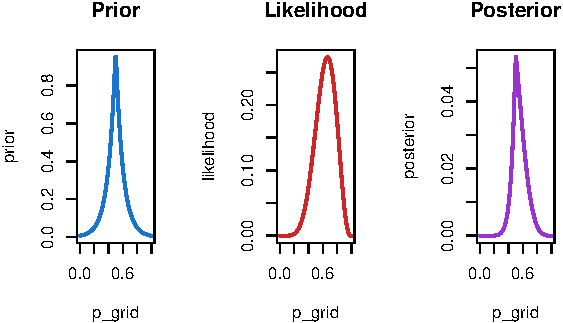
\includegraphics{01-intro-bayesian-stats_files/figure-latex/unnamed-chunk-19-1}

\hypertarget{beta-verteilung}{%
\subsection{Beta Verteilung}\label{beta-verteilung}}

Da wir aber nicht immer unsere Prior Verteilungen per Hand spezifieren
können oder wollen, ist es oft ratsam, eine bekannte
Wahrscheinlichkeitsverteilung zu benutzen. Diese muss einen Wertebereich
haben, der für den zu schätzenden Parameter angemessen ist. In diesem
Fall ist dies das Interval \(\left(0, 1\right)\).

Die Familie von Verteilungen, die hier in Frage kommen, sind die
\href{https://de.wikipedia.org/wiki/Beta-Verteilung}{Beta-Verteilungen}.
Diese haben zwei Parameter, \(\alpha\) und \(\beta\), welche als
Vorwissen über Erfolge und Misserfolge interpretiert werden können. Die
Anzahl Versuche ist somit \(\alpha + \beta\). Diese Familie von
Verteilungen kann je Nach Wahl der beiden Parameter unterschiedliche
Formen annehmen. In Grafik @ref(fig:betadists) sind einige dargestellt.

\begin{Shaded}
\begin{Highlighting}[]
\NormalTok{length }\OtherTok{\textless{}{-}} \FloatTok{1e4}
\NormalTok{d }\OtherTok{\textless{}{-}} \FunctionTok{crossing}\NormalTok{(}\AttributeTok{shape1 =} \FunctionTok{c}\NormalTok{(.}\DecValTok{1}\NormalTok{, }\DecValTok{1}\SpecialCharTok{:}\DecValTok{4}\NormalTok{),}
           \AttributeTok{shape2 =} \FunctionTok{c}\NormalTok{(.}\DecValTok{1}\NormalTok{, }\DecValTok{1}\SpecialCharTok{:}\DecValTok{4}\NormalTok{)) }\SpecialCharTok{\%\textgreater{}\%}
  \FunctionTok{expand}\NormalTok{(}\FunctionTok{nesting}\NormalTok{(shape1, shape2),}
         \AttributeTok{x =} \FunctionTok{seq}\NormalTok{(}\AttributeTok{from =} \DecValTok{0}\NormalTok{, }\AttributeTok{to =} \DecValTok{1}\NormalTok{, }\AttributeTok{length.out =}\NormalTok{ length)) }\SpecialCharTok{\%\textgreater{}\%} 
  \FunctionTok{mutate}\NormalTok{(}\AttributeTok{a =} \FunctionTok{str\_c}\NormalTok{(}\StringTok{"a = "}\NormalTok{, shape1),}
         \AttributeTok{b =} \FunctionTok{str\_c}\NormalTok{(}\StringTok{"b = "}\NormalTok{, shape2),}
         \AttributeTok{group =} \FunctionTok{rep}\NormalTok{(}\DecValTok{1}\SpecialCharTok{:}\NormalTok{length, }\AttributeTok{each =} \DecValTok{25}\NormalTok{))}
\end{Highlighting}
\end{Shaded}

\begin{Shaded}
\begin{Highlighting}[]
\NormalTok{d }\SpecialCharTok{\%\textgreater{}\%} 
  \FunctionTok{ggplot}\NormalTok{(}\FunctionTok{aes}\NormalTok{(}\AttributeTok{x =}\NormalTok{ x, }\AttributeTok{group =}\NormalTok{ group)) }\SpecialCharTok{+}
  
  \FunctionTok{geom\_line}\NormalTok{(}\FunctionTok{aes}\NormalTok{(}\AttributeTok{y =} \FunctionTok{dbeta}\NormalTok{(x, }\AttributeTok{shape1 =}\NormalTok{ shape1, }\AttributeTok{shape2 =}\NormalTok{ shape2)),}
            \AttributeTok{color =} \StringTok{"steelblue4"}\NormalTok{, }\AttributeTok{size =} \FloatTok{1.1}\NormalTok{) }\SpecialCharTok{+}
  \FunctionTok{scale\_x\_continuous}\NormalTok{(}\FunctionTok{expression}\NormalTok{(theta), }\AttributeTok{breaks =} \FunctionTok{c}\NormalTok{(}\DecValTok{0}\NormalTok{, .}\DecValTok{5}\NormalTok{, }\DecValTok{1}\NormalTok{)) }\SpecialCharTok{+}
  \FunctionTok{coord\_cartesian}\NormalTok{(}\AttributeTok{ylim =} \FunctionTok{c}\NormalTok{(}\DecValTok{0}\NormalTok{, }\DecValTok{3}\NormalTok{)) }\SpecialCharTok{+}
  \FunctionTok{labs}\NormalTok{(}\AttributeTok{title =} \StringTok{"Beispiele von Beta Verteilungen"}\NormalTok{,}
       \AttributeTok{y =} \FunctionTok{expression}\NormalTok{(}\FunctionTok{p}\NormalTok{(theta}\SpecialCharTok{*}\StringTok{"|"}\SpecialCharTok{*}\NormalTok{a}\SpecialCharTok{*}\StringTok{", "}\SpecialCharTok{*}\NormalTok{b))) }\SpecialCharTok{+}
  \FunctionTok{theme}\NormalTok{(}\AttributeTok{panel.grid =} \FunctionTok{element\_blank}\NormalTok{()) }\SpecialCharTok{+}
  \FunctionTok{facet\_grid}\NormalTok{(b}\SpecialCharTok{\textasciitilde{}}\NormalTok{a)}
\end{Highlighting}
\end{Shaded}

\begin{figure}
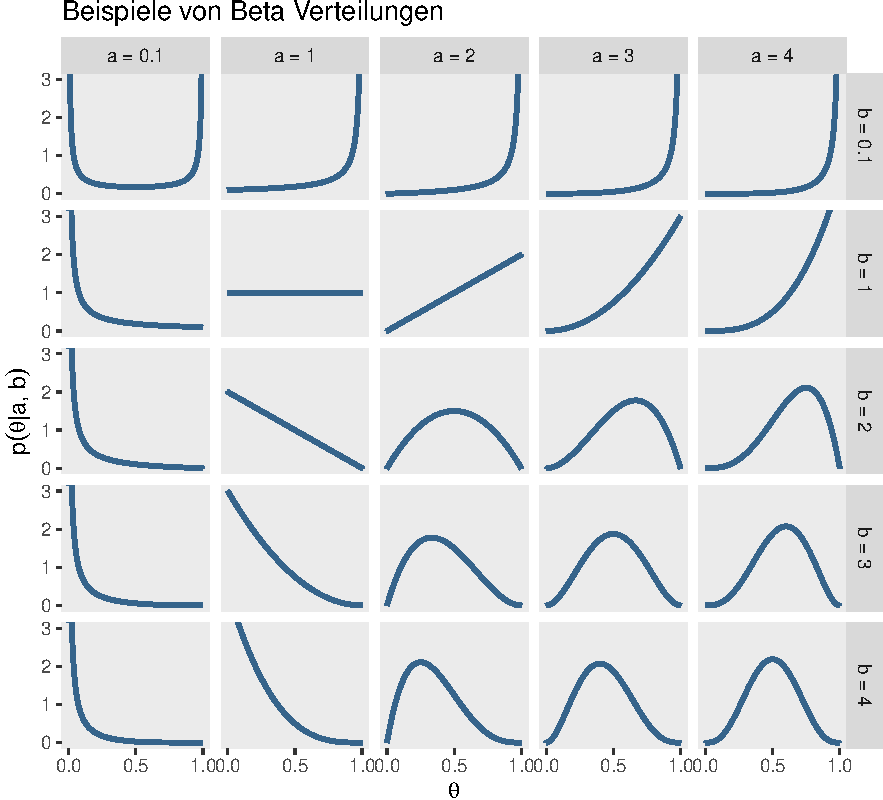
\includegraphics{01-intro-bayesian-stats_files/figure-latex/betadists-1} \caption[Beta Verteilungen]{Beta Verteilungen}\label{fig:betadists}
\end{figure}

Die uniforme Verteilung erhalten wir, wenn wir \(\alpha = \beta = 1\)
setzen. Wenn wir \(\alpha = \beta = 4\) setzen, erhalten wir eine
Verteilung mit Erwartungswert \(0.5\)---dies ist der Fall für alle
Verteilungen in denen die beiden Parameter denselben Wert annehmen. Wenn
wir ausdrücken wollen, dass wir A für die bessere Spielerin als B
halten, dann wählen wir \(\alpha > \beta\).

Die Verteilungsfunktionen heissen in R \texttt{dbeta()},
\texttt{pbeta()}, \texttt{qbeta()} und \texttt{rbeta()}. Die Parameter
\(\alpha\) und \(\beta\) heissen ganz einfach \texttt{shape1} und
\texttt{shape2}.

\begin{Shaded}
\begin{Highlighting}[]
\NormalTok{prior4 }\OtherTok{\textless{}{-}} \FunctionTok{dbeta}\NormalTok{(}\AttributeTok{x =}\NormalTok{ p\_grid, }\AttributeTok{shape1 =} \DecValTok{20}\NormalTok{, }\AttributeTok{shape2 =} \DecValTok{4}\NormalTok{)}
\FunctionTok{compute\_posterior}\NormalTok{(likelihood, prior4)}
\end{Highlighting}
\end{Shaded}

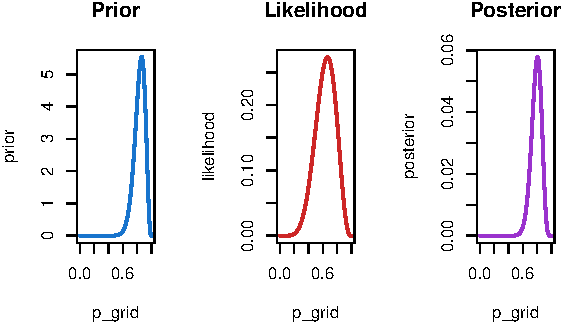
\includegraphics{01-intro-bayesian-stats_files/figure-latex/unnamed-chunk-21-1}

Wenn wir überzeugt wären, dass B besser ist, dann hätten wir vielleicht
diesen Prior:

\begin{Shaded}
\begin{Highlighting}[]
\NormalTok{prior5 }\OtherTok{\textless{}{-}} \FunctionTok{dbeta}\NormalTok{(}\AttributeTok{x =}\NormalTok{ p\_grid, }\AttributeTok{shape1 =} \DecValTok{4}\NormalTok{, }\AttributeTok{shape2 =} \DecValTok{20}\NormalTok{)}
\FunctionTok{compute\_posterior}\NormalTok{(likelihood, prior5)}
\end{Highlighting}
\end{Shaded}

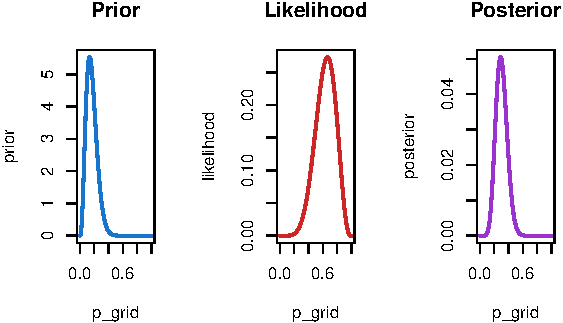
\includegraphics{01-intro-bayesian-stats_files/figure-latex/unnamed-chunk-22-1}
\#\# Einfluss des Priors auf den Posterior

Die obigen Beispiele illustrieren, dass die Prior-Verteilung einen
grossen Einfluss auf die Schätzung haben kann. Deshalb ist bei der Wahl
der Prior Vorsichtig geboten; vor allem wenn es darum geht, Parameter in
statistischen Modellen zu schätzen, wollen wir oft sogenannte
\textbf{non-informative} Priors, welche keine nennenswerten Einfluss auf
die Schätzung haben.

Probieren Sie ein ähnliches Beispiel als interaktive Webapp:
\href{https://tellmi.psy.lmu.de/felix/BayesLessons/BayesianLesson1.Rmd}{A
First Lesson in Bayesian Inference}

\hypertarget{schuxe4tzmethoden}{%
\subsection{Schätzmethoden}\label{schuxe4tzmethoden}}

Die Methode, welche wir oben angewandt haben, nennt sich
``grid-search.'' Dies bezieht sich auf den Prior---wir haben einen
Vektor von Priorwerten definiert, und jeden Punkt mit der Likelihood
multipliziert, in direkter Anwendung von Bayes' Theorem. Dies ist für
dieses kleine Problem sehr gut möglich. Daneben gibt es für dieses
Beispiel auch die analytische Lösung. Die Beta-Prior-Verteilung kann mit
den beobachteten Erfolgen und Versuchen updated werden, um eine neue
Beta-Verteilung mit den Parametern \(k + \alpha\) und \(n - k + \beta\).

Mehr dazu einem Blog Post.

Nun kommen diese beiden Ansatz für die meisten Datenanalyseprobleme
nicht in Frage. Die analytische Lösung ist nicht möglich, und die
grid-search Methode ist nicht in endlicher Zeit durchführbar. In diesem
Fall sind wir auf approximative Methoden angewiesen. Eine Variante,
welche die Posterior-Verteilung durch Ziehen von Zufallszahlen
exploriert, heisst Markov CHain Monte Carlo. Davon gibt es wiederum
verschiedene Varianten.

\hypertarget{stan}{%
\subsection{Stan}\label{stan}}

Ein Algorithmus, welcher als \emph{state-of-the-art} gilt, heisst
Hamiltonian Monte Carlo, und eine spezielle Variante davon heisst
\emph{NUTS} (No-U-Turn Sampler). Auf diese Inferenzmethode ist die
probabilistische Programmiersprache Stan spezialisiert.

Wir werden in dieser Veranstaltung selten Stan direkt verwenden, da es
mittlerweile gute R Packages gibt, mit denen die Bedienung von Stan sehr
einfach geworden ist. Ich halte es jedoch für pädagogisch wertvoll, wenn
wir uns zumindest dieses Beta-Binomial Besipiel in Stan anschauen.

Die Vorgehensweise ist genauso, wie oben beschrieben: wir schreiben
zuerst ein probabilistischen Model\footnote{Dies nennt man ein
  generatives Modell} auf, und bedingen dann auf die beobachteten Daten.

Das Modell wird in der Stan Sprache geschrieben. Wir verwenden hier
einen \texttt{Beta(4,\ 4)} Prior.

\begin{verbatim}
data {
  int<lower=0> n; // number of games
  int<lower=0> k; // number of wins
  
}

parameters {
  real<lower=0, upper=1> theta;
}

model {
  theta ~ beta(4, 4);
  k ~ binomial(n, theta);
}
\end{verbatim}

Dieser Code wird in einem File mit dem Suffix \texttt{.stan}
gespeichert.

Ich nenne das Stan File \texttt{binomial-model.stan}.

Wir laden das Package \href{https://mc-stan.org/rstan/}{rstan}, das R
Interface zu Stan.

\begin{Shaded}
\begin{Highlighting}[]
\FunctionTok{library}\NormalTok{(rstan)}
\end{Highlighting}
\end{Shaded}

Dann definieren wir die beobachteten Daten:

\begin{Shaded}
\begin{Highlighting}[]
\NormalTok{stan\_data }\OtherTok{\textless{}{-}} \FunctionTok{list}\NormalTok{(}
  \AttributeTok{n =} \DecValTok{9}\NormalTok{,}
  \AttributeTok{k =} \DecValTok{6}
\NormalTok{)}
\end{Highlighting}
\end{Shaded}

Und benutzen die Funktion \texttt{stan()}, um die Posterior-Verteilung
zu sampeln.

\begin{Shaded}
\begin{Highlighting}[]
\NormalTok{fit }\OtherTok{\textless{}{-}} \FunctionTok{stan}\NormalTok{(}\AttributeTok{file =} \StringTok{"../binomial{-}model.stan"}\NormalTok{,  }\CommentTok{\# Stan program}
            \AttributeTok{data =}\NormalTok{ stan\_data,    }\CommentTok{\# named list of data}
            \AttributeTok{chains =} \DecValTok{4}\NormalTok{,          }\CommentTok{\# number of Markov chains}
            \AttributeTok{iter =} \DecValTok{2000}\NormalTok{,         }\CommentTok{\# total number of iterations per chain}
            \AttributeTok{cores =} \DecValTok{4}\NormalTok{)           }\CommentTok{\# number of cores (could use one per chain)}
\end{Highlighting}
\end{Shaded}

\begin{Shaded}
\begin{Highlighting}[]
\FunctionTok{print}\NormalTok{(fit)}
\end{Highlighting}
\end{Shaded}

\begin{verbatim}
## Inference for Stan model: binomial-model.
## 4 chains, each with iter=2000; warmup=1000; thin=1; 
## post-warmup draws per chain=1000, total post-warmup draws=4000.
## 
##         mean se_mean   sd   2.5%    25%    50%    75%  97.5% n_eff Rhat
## theta   0.59    0.00 0.12   0.35   0.51   0.59   0.67   0.80  1518    1
## lp__  -12.03    0.02 0.71 -14.07 -12.22 -11.76 -11.57 -11.52  1451    1
## 
## Samples were drawn using NUTS(diag_e) at Wed Mar  3 10:02:03 2021.
## For each parameter, n_eff is a crude measure of effective sample size,
## and Rhat is the potential scale reduction factor on split chains (at 
## convergence, Rhat=1).
\end{verbatim}

\begin{Shaded}
\begin{Highlighting}[]
\FunctionTok{traceplot}\NormalTok{(fit)}
\end{Highlighting}
\end{Shaded}

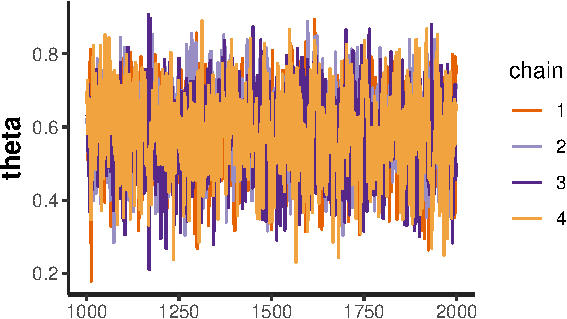
\includegraphics{01-intro-bayesian-stats_files/figure-latex/unnamed-chunk-28-1}

\begin{Shaded}
\begin{Highlighting}[]
\NormalTok{bayesplot}\SpecialCharTok{::}\FunctionTok{mcmc\_intervals}\NormalTok{(fit, }\StringTok{"theta"}\NormalTok{)}
\end{Highlighting}
\end{Shaded}

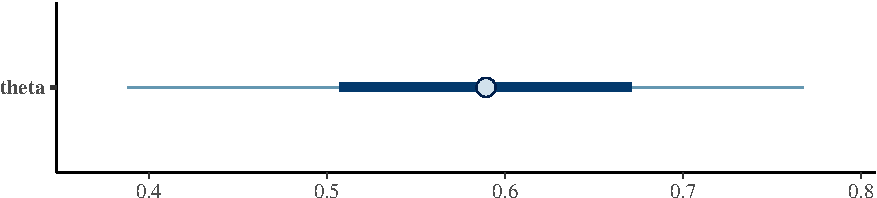
\includegraphics{01-intro-bayesian-stats_files/figure-latex/unnamed-chunk-29-1}

\begin{Shaded}
\begin{Highlighting}[]
\NormalTok{theta }\OtherTok{\textless{}{-}} \FunctionTok{extract}\NormalTok{(fit, }\AttributeTok{pars =} \FunctionTok{c}\NormalTok{(}\StringTok{"theta"}\NormalTok{))}\SpecialCharTok{$}\NormalTok{theta}
\FunctionTok{hist}\NormalTok{(theta)}
\end{Highlighting}
\end{Shaded}

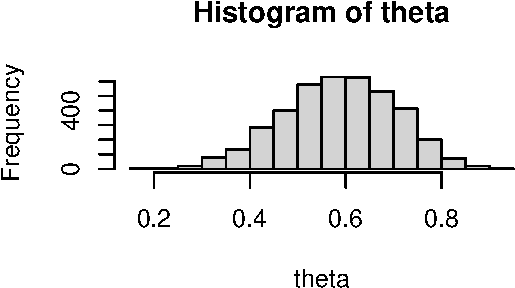
\includegraphics{01-intro-bayesian-stats_files/figure-latex/unnamed-chunk-30-1}

\hypertarget{brms}{%
\subsection{brms}\label{brms}}

\begin{Shaded}
\begin{Highlighting}[]
\FunctionTok{library}\NormalTok{(brms)}
\end{Highlighting}
\end{Shaded}

\begin{Shaded}
\begin{Highlighting}[]
\NormalTok{data }\OtherTok{\textless{}{-}} \FunctionTok{tibble}\NormalTok{(}\AttributeTok{k =} \DecValTok{6}\NormalTok{, }\AttributeTok{n =} \DecValTok{9}\NormalTok{)}
\end{Highlighting}
\end{Shaded}

\begin{Shaded}
\begin{Highlighting}[]
\NormalTok{priors }\OtherTok{\textless{}{-}} \FunctionTok{prior}\NormalTok{(}\FunctionTok{beta}\NormalTok{(}\DecValTok{4}\NormalTok{, }\DecValTok{4}\NormalTok{), }\AttributeTok{class =}\NormalTok{ b, }\AttributeTok{lb =} \DecValTok{0}\NormalTok{, }\AttributeTok{ub =} \DecValTok{1}\NormalTok{)}

\NormalTok{m1 }\OtherTok{\textless{}{-}} \FunctionTok{brm}\NormalTok{(k }\SpecialCharTok{|} \FunctionTok{trials}\NormalTok{(n) }\SpecialCharTok{\textasciitilde{}} \DecValTok{0} \SpecialCharTok{+}\NormalTok{ Intercept, }\AttributeTok{family =} \FunctionTok{binomial}\NormalTok{(}\AttributeTok{link =} \StringTok{"identity"}\NormalTok{),}
          \AttributeTok{prior =}\NormalTok{ priors,}
          \AttributeTok{data =}\NormalTok{ data,}
          \AttributeTok{control =} \FunctionTok{list}\NormalTok{(}\AttributeTok{adapt\_delta =} \FloatTok{0.9}\NormalTok{),}
          \AttributeTok{file =} \StringTok{"../models/binomial{-}2"}\NormalTok{)}
\end{Highlighting}
\end{Shaded}

\begin{Shaded}
\begin{Highlighting}[]
\FunctionTok{plot}\NormalTok{(m1)}
\end{Highlighting}
\end{Shaded}

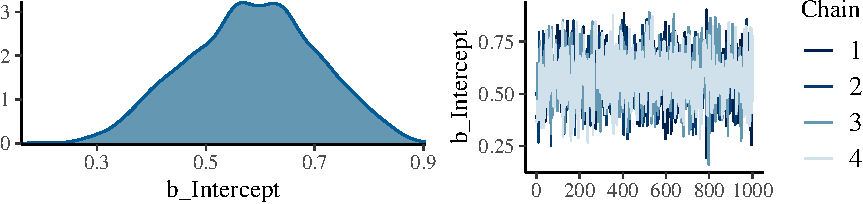
\includegraphics{01-intro-bayesian-stats_files/figure-latex/unnamed-chunk-34-1}

\hypertarget{posterior-verteilungen-zusammenfassen}{%
\subsection{Posterior-Verteilungen
zusammenfassen}\label{posterior-verteilungen-zusammenfassen}}

Wir erhalten mit Bayesianischer Inferenz zwar Posterior-Verteilungen,
aber oftmals wollen wir diese zusammen, damit wir eine Entscheidung
fällen können.

Dies wird häufig anhand bestimmter Kennzahlen gemacht. Z.B. können wir
den Mittelwert oder Median und eine Ober- und Untergrenze wählen. Ein
solches Interval wird \emph{credible interval} genannt. Häufig wird ein
\(95\%\) credible interval angegeben, aber es hindert uns nichts daran,
ein \(50\%\) oder \(80\%\) credible interval zu benutzen. Mit der
\texttt{median\_qi()} vom Package \texttt{tidybayes} können wir das
\texttt{.width} Argument benutzen:

\begin{Shaded}
\begin{Highlighting}[]
\FunctionTok{library}\NormalTok{(tidybayes)}
\end{Highlighting}
\end{Shaded}

\begin{verbatim}
## 
## Attaching package: 'tidybayes'
\end{verbatim}

\begin{verbatim}
## The following objects are masked from 'package:brms':
## 
##     dstudent_t, pstudent_t, qstudent_t, rstudent_t
\end{verbatim}

\begin{Shaded}
\begin{Highlighting}[]
\NormalTok{m1 }\SpecialCharTok{\%\textgreater{}\%}
  \FunctionTok{spread\_draws}\NormalTok{(b\_Intercept) }\SpecialCharTok{\%\textgreater{}\%} 
  \FunctionTok{median\_qi}\NormalTok{(}\AttributeTok{.width =} \FunctionTok{c}\NormalTok{(.}\DecValTok{50}\NormalTok{, .}\DecValTok{80}\NormalTok{, .}\DecValTok{95}\NormalTok{)) }\SpecialCharTok{\%\textgreater{}\%} 
\NormalTok{  kableExtra}\SpecialCharTok{::}\FunctionTok{kbl}\NormalTok{()}
\end{Highlighting}
\end{Shaded}

\begin{tabular}[t]{r|r|r|r|l|l}
\hline
b\_Intercept & .lower & .upper & .width & .point & .interval\\
\hline
0.5885875 & 0.5025237 & 0.6682483 & 0.50 & median & qi\\
\hline
0.5885875 & 0.4231849 & 0.7428155 & 0.80 & median & qi\\
\hline
0.5885875 & 0.3514341 & 0.8102628 & 0.95 & median & qi\\
\hline
\end{tabular}

Mit \texttt{mean\_qi()} erhalten wir Mittelwert und credible intervals.

Um die Posterior-Verteilung zu visualisieren, können wir die Verteilung
mit einem credible interval kombinieren.

\begin{Shaded}
\begin{Highlighting}[]
\NormalTok{m1 }\SpecialCharTok{\%\textgreater{}\%}
  \FunctionTok{spread\_draws}\NormalTok{(b\_Intercept) }\SpecialCharTok{\%\textgreater{}\%}
  \FunctionTok{ggplot}\NormalTok{(}\FunctionTok{aes}\NormalTok{(}\AttributeTok{x =}\NormalTok{ b\_Intercept)) }\SpecialCharTok{+}
  \FunctionTok{stat\_halfeye}\NormalTok{(}\AttributeTok{.width =} \FunctionTok{c}\NormalTok{(.}\DecValTok{50}\NormalTok{, .}\DecValTok{80}\NormalTok{, .}\DecValTok{95}\NormalTok{))}
\end{Highlighting}
\end{Shaded}

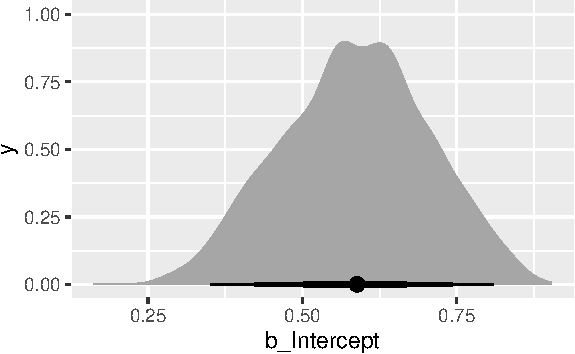
\includegraphics{01-intro-bayesian-stats_files/figure-latex/unnamed-chunk-37-1}

Was ist der Unterschied zwischen einem \textbf{Konfidenzintervall} und
einem \textbf{credible interval}? Welches Intervall würden Sie
verwenden, um eine Wahrscheinlichkeitsaussage über einen Parameter zu
machen?

\hypertarget{weiterfuxfchrende-literatur}{%
\subsection{Weiterführende
Literatur}\label{weiterfuxfchrende-literatur}}

Etz and Vandekerckhove (2018) bieten eine sehr gründliche Einführung,
mit vielen (Harry Potter-themed) Beispielen. Schoot et al. (2014) ist
ebenfalls eine sehr gründliche Einführung. Eine empfehlenswerte
Übersicht über Literatur, vor allem in Bezug auf Psychologie, geben Etz
et al. (2016).

Das Buch von (Kruschke 2015) ist ein gutes Lehrbuch, obwohl der R Code
nicht unbedingt sehr benutzerfreundlich ist.

Mein Favorit ist McElreath (2020).

\hypertarget{refs}{}
\begin{CSLReferences}{1}{0}
\leavevmode\hypertarget{ref-etzHowBecomeBayesian2016}{}%
Etz, Alexander, Quentin Frederik Gronau, Fabian Dablander, Peter
Edelsbrunner, and Beth Baribault. 2016. {``How to Become a {Bayesian} in
Eight Easy Steps: {An} Annotated Reading List,''} August.
\url{https://doi.org/10.31234/osf.io/ph6sw}.

\leavevmode\hypertarget{ref-etzIntroductionBayesianInference2018}{}%
Etz, Alexander, and Joachim Vandekerckhove. 2018. {``Introduction to
{Bayesian Inference} for {Psychology}.''} \emph{Psychonomic Bulletin \&
Review} 25 (1): 5--34. \url{https://doi.org/10.3758/s13423-017-1262-3}.

\leavevmode\hypertarget{ref-gigerenzerMindlessStatistics2004}{}%
Gigerenzer, Gerd. 2004. {``Mindless Statistics.''} \emph{The Journal of
Socio-Economics} 33 (5): 587--606.
\url{https://doi.org/10.1016/j.socec.2004.09.033}.

\leavevmode\hypertarget{ref-gigerenzerStatisticalRitualsReplication2018a}{}%
---------. 2018. {``Statistical {Rituals}: {The Replication Delusion}
and {How We Got There}.''} \emph{Advances in Methods and Practices in
Psychological Science} 1 (2): 198--218.
\url{https://doi.org/10.1177/2515245918771329}.

\leavevmode\hypertarget{ref-hoekstraRobustMisinterpretationConfidence2014}{}%
Hoekstra, Rink, Richard D. Morey, Jeffrey N. Rouder, and Eric-Jan
Wagenmakers. 2014. {``Robust Misinterpretation of Confidence
Intervals.''} \emph{Psychonomic Bulletin \& Review} 21 (5): 1157--64.
\url{https://doi.org/10.3758/s13423-013-0572-3}.

\leavevmode\hypertarget{ref-kruschkeDoingBayesianData2015}{}%
Kruschke, John. 2015. \emph{Doing Bayesian Data Analysis (Second
Edition)}. {Boston}: {Academic Press}.

\leavevmode\hypertarget{ref-mcelreathStatisticalRethinkingBayesian2020}{}%
McElreath, R. 2020. \emph{Statistical Rethinking: {A} Bayesian Course
with Examples in r and Stan}. A Chapman \& Hall Book. {CRC Press}.
\url{https://books.google.ch/books?id=Ie2vxQEACAAJ}.

\leavevmode\hypertarget{ref-schootGentleIntroductionBayesian2014}{}%
Schoot, Rens van de, David Kaplan, Jaap Denissen, Jens B. Asendorpf,
Franz J. Neyer, and Marcel A. G. van Aken. 2014. {``A {Gentle
Introduction} to {Bayesian Analysis}: {Applications} to {Developmental
Research}.''} \emph{Child Development} 85 (3): 842--60.
\url{https://doi.org/10.1111/cdev.12169}.

\leavevmode\hypertarget{ref-wagenmakersPracticalSolutionPervasive2007}{}%
Wagenmakers, Eric-Jan. 2007. {``A Practical Solution to the Pervasive
Problems of p Values.''} \emph{Psychonomic Bulletin \& Review} 14 (5):
779--804. \url{https://doi.org/10.3758/BF03194105}.

\leavevmode\hypertarget{ref-wassersteinASAStatementPValues2016}{}%
Wasserstein, Ronald L., and Nicole A. Lazar. 2016. {``The {ASA
Statement} on p-{Values}: {Context}, {Process}, and {Purpose}.''}
\emph{The American Statistician} 70 (2): 129--33.
\url{https://doi.org/10.1080/00031305.2016.1154108}.

\end{CSLReferences}



\end{document}
